\chapter{Datasets and Triggers}
\label{chap:Samples}

\section{Triggers}
The data for this search are collected using several dilepton triggers. The double electron trigger requires two electrons with \pt thresholds of 17\,\GeV on the leading electron and 12\,\GeV on the sub-leading electron. The double muon trigger requires two muons with \pt thresholds of 17 and 8\,\GeV on the leading and sub-leading muons, respectively. We use two muon/electron cross triggers, one of which requires a 17\,\GeV muon and a 12\,\GeV electron, while the other requires a 17\,\GeV electron and a 8\,\GeV muon.

We use the data sets listed in Table~\ref{tab:DataSamples}, masked using the ``Golden JSON file'' \path{/afs/cern.ch/cms/CAF/CMSCOMM/COMM_DQM/certification/Collisions15/13TeV/Reprocessing/Cert_13TeV_16Dec2015ReReco_Collisions15_25ns_JSON_v2.txt}.

\begin{table}
\centering
\caption{Data samples} \label{tab:DataSamples}
\begin{tabular}{c c c}
\hline\hline
Primary Dataset & Reconstruction labels & L [fb$^{-1}$]\\
\hline
DoubleEG & Run2015D-05Oct2015-v1 & 0.59\\
DoubleEG & Run2015D-PromptReco-v4 & 1.66\\
\hline
DoubleMuon & Run2015D-05Oct2015-v1 & 0.59\\
DoubleMuon & Run2015D-PromptReco-v4 & 1.66\\
\hline
MuonEG & Run2015D-05Oct2015-v1 & 0.59\\
MuonEG & Run2015D-PromptReco-v4 & 1.66\\
\end{tabular}
\end{table}


\section{Background MC samples}
For background determination, we use the Monte Carlo samples listed in Table~\ref{tab:MCSamples}.

\begin{sidewaystable}
\centering
\caption{Background MC samples} \label{tab:MCSamples}
\begin{tabular}{p{14cm} l c c c l}
\hline\hline
Sample & xsec [pb] & L [pb$^{-1}$] & No. events read\\
\hline
/WZTo3LNu\_TuneCUETP8M1\_13TeV-powheg-pythia8 \newline /RunIISpring15DR74-Asympt25ns\_MCRUN2\_74\_V9-v1/MINIAODSIM	& 4.42965	& 447169	& 1.9808e+06\\
\hline
/WZJets\_TuneCUETP8M1\_13TeV-amcatnloFXFX-pythia8/ \newline RunIISpring15MiniAODv2-74X\_mcRun2\_asymptotic\_v2-v1/MINIAODSIM	& 5.263	& 2.37929e+06	& 1.252220e+07\\
\hline
/ZZTo4L\_13TeV-amcatnloFXFX-pythia8 \newline /RunIISpring15DR74-Asympt25nsRaw\_MCRUN2\_74\_V9-v1/MINIAODSIM	& 1.212	& 8.71378e+06	& 1.05611e+07\\
\hline
/TTTo2L2Nu\_13TeV-powheg \newline /RunIISpring15DR74-Asympt25ns\_MCRUN2\_74\_V9-v1/MINIAODSIM	& 87.31	& 69711.1	& 4.997e+06\\ 
\hline
/TTWJetsToLNu\_TuneCUETP8M1\_13TeV-amcatnloFXFX-madspin-pythia8 \newline /RunIISpring15DR74-Asympt25ns\_MCRUN2\_74\_V9-v1/MINIAODSIM	& 0.2043	& 1.23792e+06	& 252908\\
\hline
/TTZToLLNuNu\_M-10\_TuneCUETP8M1\_13TeV-amcatnlo-pythia8 \newline /RunIISpring15DR74-Asympt25ns\_MCRUN2\_74\_V9-v1/MINIAODSIM	& 0.2529	& 1.57374e+06	& 398000\\
\hline
/WWZ\_TuneCUETP8M1\_13TeV-amcatnlo-pythia8/ \newline RunIISpring15MiniAODv2-74X\_mcRun2\_asymptotic\_v2-v1/MINIAODSIM	& 0.1651	& 1.51423e+06	& 250000\\
\hline
/WZZ\_TuneCUETP8M1\_13TeV-amcatnlo-pythia8/ \newline RunIISpring15MiniAODv2-74X\_mcRun2\_asymptotic\_v2-v1/MINIAODSIM	& 0.05565	& 4.49236e+06	& 250000\\
\hline
/ZZZ\_TuneCUETP8M1\_13TeV-amcatnlo-pythia8/ \newline RunIISpring15MiniAODv2-74X\_mcRun2\_asymptotic\_v2-v1/MINIAODSIM	& 0.01398	& 1.78827e+07	& 250000\\
\hline
/GluGluHToZZTo4L\_M125\_13TeV\_powheg\_JHUgen\_pythia8 \newline /RunIISpring15MiniAODv2-74X\_mcRun2\_asymptotic\_v2-v1/MINIAODSIM	& 0.01212	& 4.10891e+07	& 498000\\
\hline
/VBF\_HToZZTo4L\_M125\_13TeV\_powheg\_JHUgen\_pythia8 \newline /RunIISpring15MiniAODv2-74X\_mcRun2\_asymptotic\_v2-v1/MINIAODSIM	& 0.001034	& 4.73362e+08	& 489456\\
\hline
/DYJetsToLL\_M-10to50\_TuneCUETP8M1\_13TeV-amcatnloFXFX-pythia8 \newline /RunIISpring15MiniAODv2-74X\_mcRun2\_asymptotic\_v2-v1/MINIAODSIM	& 18610	& 1613.2	& 3.002156+e07\\
\hline
/DYJetsToLL\_M-50\_TuneCUETP8M1\_13TeV-amcatnloFXFX-pythia8 \newline /RunIISpring15MiniAODv2-74X\_mcRun2\_asymptotic\_v2-v1/MINIAODSIM	& 6025.2	& 4771.29	& 2.874797+e07\\

\end{tabular}
\end{sidewaystable}

Some MC generators provide events with negative weights to allow for a more precise prediction of higher-order contributions. Where provided, we take these negative weights into account.

For each MC sample, the pile-up distribution is compared to the distribution in data. Weights are applied on a per-event basis so that the distribution matches for each sample.

We also correct the pile-up dependence of our data-driven background estimate using the linear fit $0.773 + 0.0218 \cdot n_\textrm{vertex}$. As a result of these weights, the background shape of the $n_\textrm{vertex}$ distribution agrees with the data. Fig.~\ref{fig:pileupWeights} shows this distribution before and after pile-up weights for events with at least three electrons or muons, without any other cuts.

\begin{figure}[h]
\begin{center}
	\begin{subfigure}[b]{.7\textwidth}
		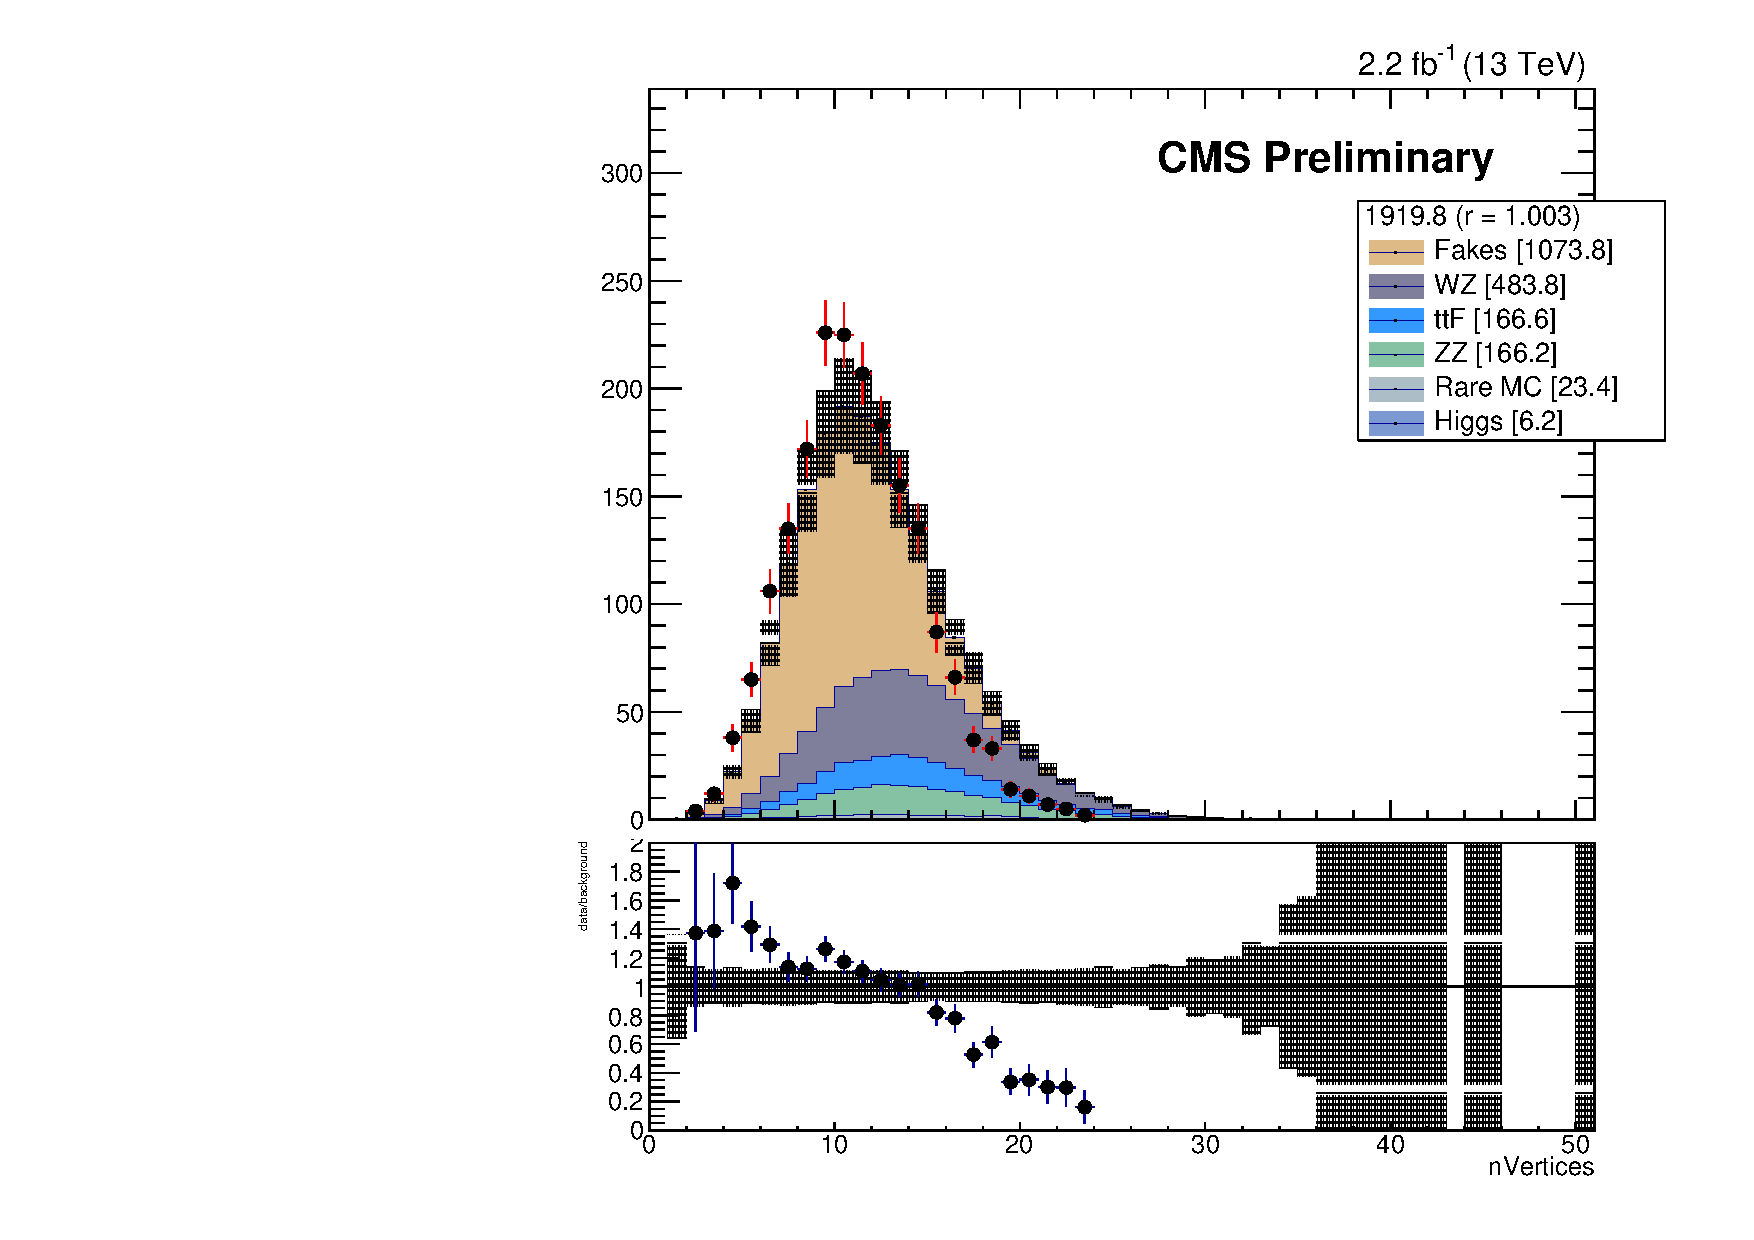
\includegraphics[width=\textwidth]{Samples/NVERTICES_Tau0-noPileupWeights}
		\caption{before pile-up weights}
	\end{subfigure}
	\begin{subfigure}[b]{.7\textwidth}
		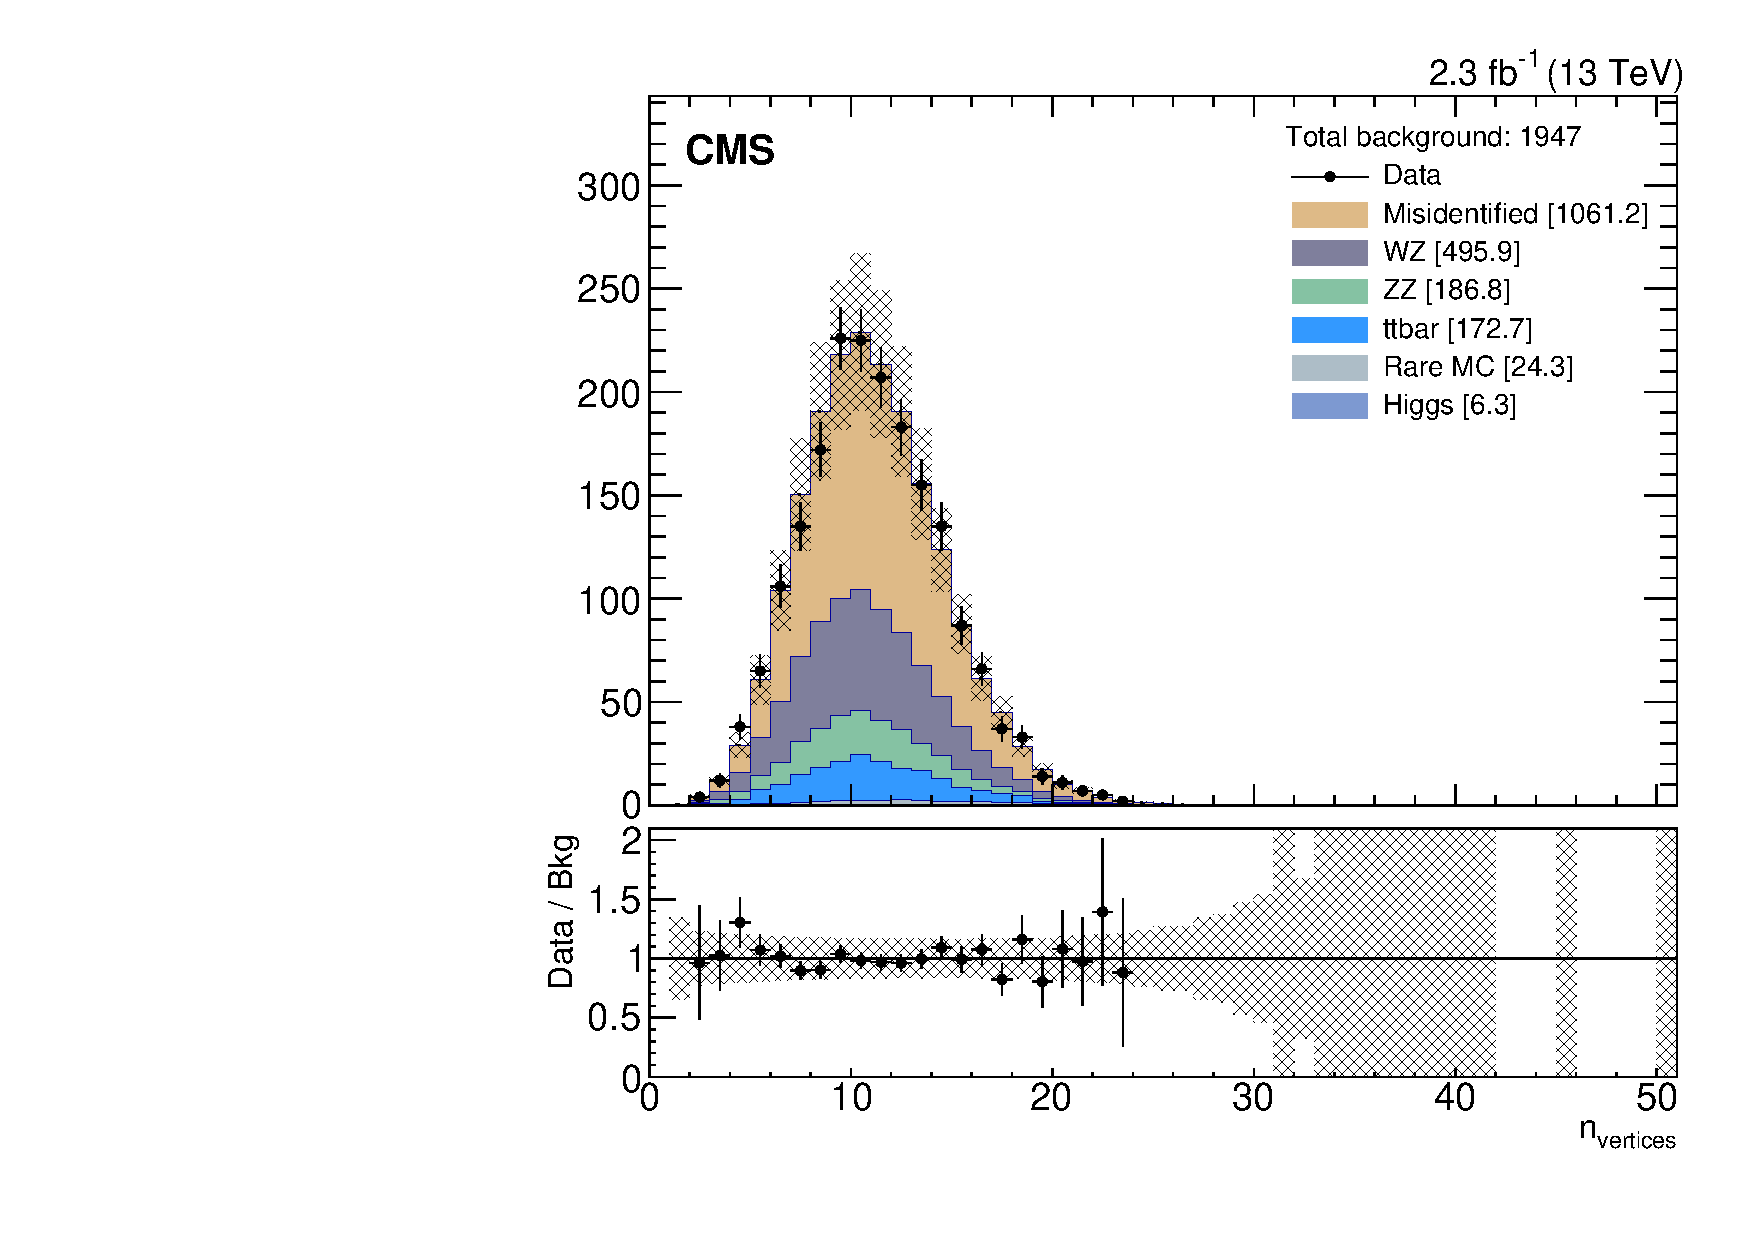
\includegraphics[width=\textwidth]{Samples/NVERTICES_Tau0}
		\caption{after pile-up weights}
	\end{subfigure}
	\caption{$n_\textrm{vertex}$ distribution for events with at least three light leptons
	\label{fig:pileupWeights}}
\end{center}
\end{figure}
